\documentclass[11pt, a4paper]{article}

\usepackage{anyfontsize}
\usepackage{txfonts} 
\usepackage{booktabs}
\usepackage{array}
\usepackage{geometry}
\usepackage{graphicx}
\graphicspath{{img/}}
\geometry{left=3cm,right=2.5cm,top=3.5cm,bottom=4cm}

%Graphics preamble
\usepackage{graphicx} %Allow you to import images
\usepackage{float} %Allow for control of float position

%Header and Footer Stuff
\pagestyle{myheadings}\markboth{page \thepage}{\emph User Manual for Mesa Mapping Robot}

%Table
\setlength{\arrayrulewidth}{0.5mm}

\begin{document}

\begin{titlepage}

\begin{center}

	\vspace{0.5 cm}
	\fontsize{35}{35}\selectfont\bf {User Manual}\\
	\vspace{0.5 cm}
	\huge{\bfseries for}\\
	\vspace{0.5 cm}
	\fontsize{35}{40}\selectfont\bf {Mesa Mapping Robot}\\
	
	\vspace{2cm}
	\Large\textbf{ Version 1.0 approved}\\
	
	\vspace{1.5cm}
	\Large\textbf {Prepared by SEP Group 19 - Spark\\
								Luo Yawen a1657343 \\
								Wei Jingwen a1671836 \\
								Wang Yuzhu a1690773 \\
								Yang Jiajun a1662541\\
								Zhang Yun a1653772}\\
		
	\vspace{2cm}
	\Large\textbf{ School of Computer Science,\\
								The University of Adelaide}\\
	\vspace{2cm}
	
	\Large\textbf{Nov 01, 2015}\\

\end{center}

\end{titlepage}

%This is table of contents stuff
\pagenumbering{roman}
\tableofcontents

%This is the version history stuff
\vspace{1cm}
\section*{Revision History}
\addcontentsline{toc}{section}{\numberline{}Revision History}
%\begin{table}
\small
\begin{tabular} 
	 {|m{3cm}|m{2cm}|m{8cm}|m{2cm}|}
	\hline
	\textbf{Name} &  \textbf{Date} & \textbf{Reason For Changes} & \textbf{Version} \\ [0.5ex]
	\hline
	Zhang Yun & 29/Oct/15 & Complete all sections & 0.1 \\ [0.5ex]
	\hline
	Zhang Yun & 31/Oct/15 & Review & 0.5 \\ [0.5ex]
	\hline
	Luo Yawen & 01/Nov/15 & Release & 1.0 \\ [0.5ex]
	\hline
\end{tabular}
%\end{table}
\cleardoublepage

\newpage


%This is main body stuff
\pagenumbering{arabic}
\setcounter{page}{1}

\section{Resources requirements}
\subsection{For PC's environment:}
\begin{itemize}
\item {JDK 1.7 installed on PC }
 \item {Ant and Make tool}
\item {OS: }Windows, MacOSX and Linux
\item {RAM: }At least 256MB
\item {Disk Space: } At least 10MB
\item {Bluetooth communication support}
\end{itemize}

\subsection{For Robot's needs:}
\begin{itemize}
\item {Robot kit: }Lego Mindstorms EV3
\item {Working plane: }A1 paper size
\item {Colour of Background: }White
\item {Colours of Deposit: } Red, yellow, blue and green
\item {Colours of Boundary and NGZ: }Black
\item {Size of Boundary and NGZ: }rectangular
\item {Size of Deposit: }circle
\end{itemize}



\section{Operations}
\indent\indent\textbf{2.1} Start up the robot by pressing the middle button.\\
\\
\indent\textbf{2.2} Join a personal area network through the Bluetooth communication.\\
\\
Note the following figures show how to connect to the robot under Windows. Please refer to the operating system documents for how to operate under other operating systems such as Linux and Mac OS.\\
\\
\indent\textbf{2.2.1} Click on the Bluetooth Icon on the tray area and click on the menu item [Join a Personal Area Network], then the following window pops up.\\

%Here we insert our figure
\begin{figure}[H]
\centering
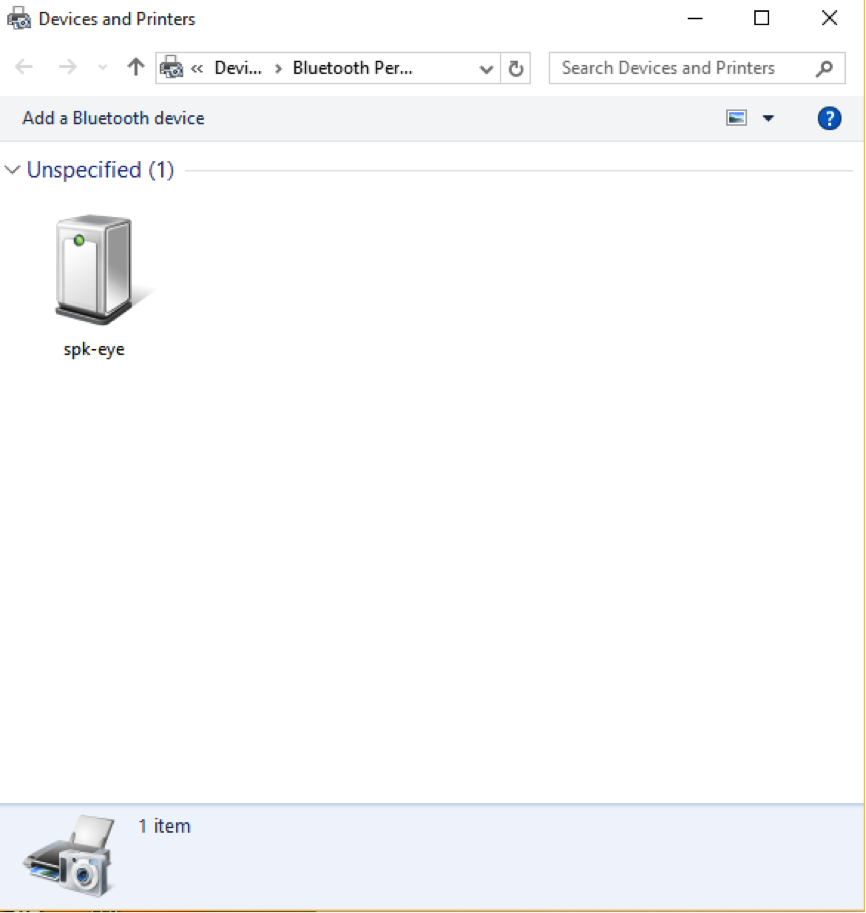
\includegraphics[height=3.3in]{UM1}
%\caption[]{}
\end{figure}

\indent\textbf{2.2.2} Right click on the chosen network on the above figure, click on [Connect using] and then [Access point]. \\
\\
\indent\textbf{2.3} Go to the project directory, run the following command to start the program on the robot.\\
 \indent \indent- make remoteRun\\
 \\
\indent\textbf{2.4} Go to the project root directory, run the following command to start the GUI program.\\
\indent \indent - make run\\
 \\
\indent\textbf{2.5} The GUI is shown as follows:\\

%Here we insert our figure
\begin{figure}[H]
\centering
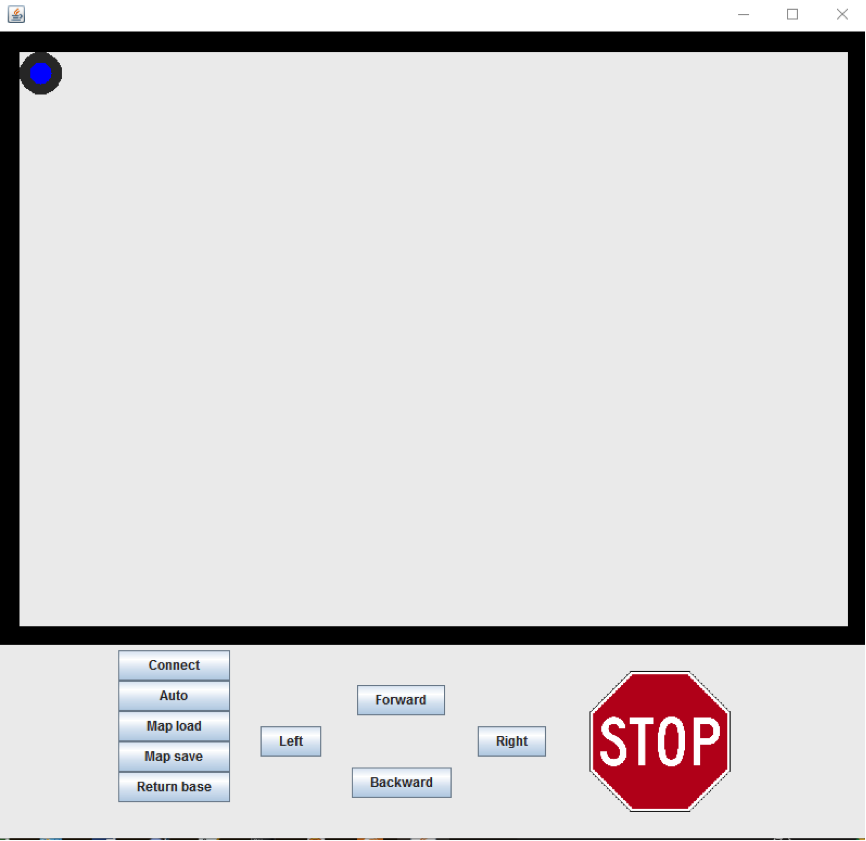
\includegraphics[height=3.2in]{UM2}
%\caption[]{}
\end{figure}

\textbf{2.5.1} The user interface is shown as the above figure, the top area shows the map and bottom area contains the command buttons.\\
\\
\indent\textbf{2.5.2} The black rectangle is the boundary of the map. The black dot on the top left corner is the origin. The blue dot is the current location of the robot.\\
\\
\indent\textbf{2.5.3} [Click] button is used to connect to the robot control program.  When the GUI is connected to the robot, you can click the disconnect button to disconnect with the robot.\\
\\
\indent\textbf{2.5.4} The default mode is manual, you can click the Auto button to switch the operation mode to automatic mode, where the robot explores the map automatically. \\
\\
\indent\textbf{2.5.5} In the manual mode, you can click on [Left], [Right], [Forward], [Backward], [stop] to turn left, turn right, move forwards, move backwards and stop respectively.\\
\\
\indent\textbf{2.5.6} In the Auto mode, the robot explores the map along lines parallel to the boundaries. The robot will detect and report deposits, obstacles, no-go-zones and base station to GUI. As a result, GUI will show those objects on the map.\\
\\
\indent\textbf{2.5.7} The [Map save] button can be clicked on to pop up the following dialog to save the current map to an XML file.\\

%Here we insert our figure
\begin{figure}[H]
\centering
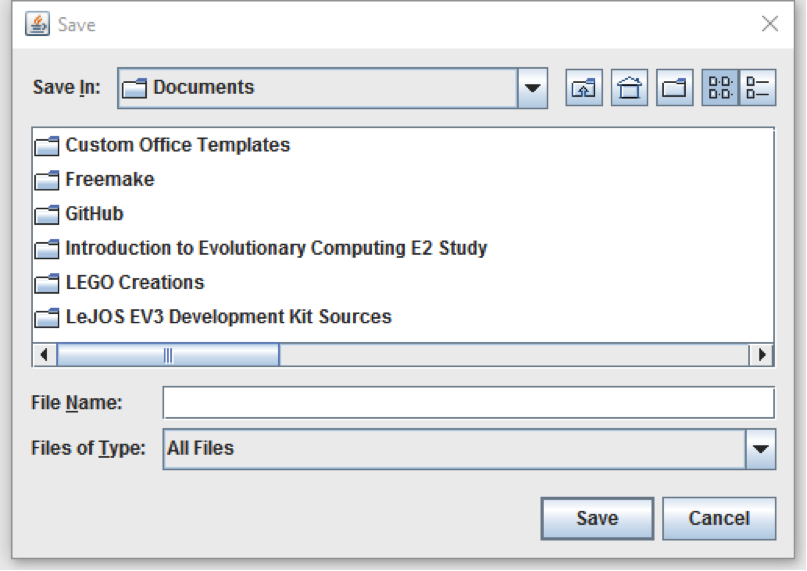
\includegraphics[height=3in]{UM3}
%\caption[]{}
\end{figure}
\newpage

\textbf{2.5.8} The [Map load] button can be clicked on to pop up the following dialog to load an XML file into the current map.\\

%Here we insert our figure
\begin{figure}[H]
\centering
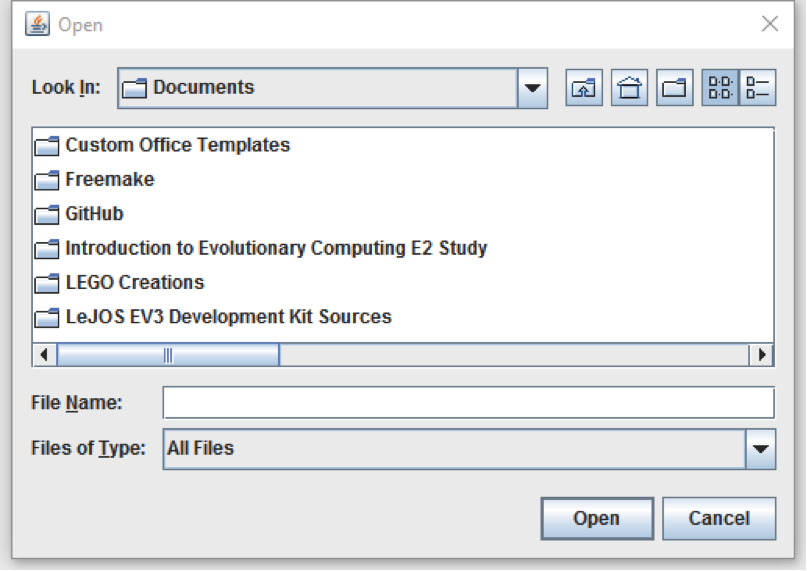
\includegraphics[height=3in]{UM4}
%\caption[]{}
\end{figure}

\end{document}